\documentclass[12pt,addpoints]{exam}
%\usepackage{enumitem}
\usepackage{amsfonts,amssymb,amsmath, amsthm}
\usepackage{graphicx}
\usepackage{systeme}
\usepackage{pgf,tikz,pgfplots}
\pgfplotsset{compat=1.15}
\usepgfplotslibrary{fillbetween}
\usepackage{mathrsfs}
\usetikzlibrary{arrows}
\usetikzlibrary{calc}
\usepackage{geometry}
\geometry{
	a4paper,
	total={170mm,257mm},
	left=15mm,
	right=15mm,
	bottom=20mm,
	top=15mm,
}
\date{June, 2023}
\pagestyle{headandfoot}
%\firstpageheadrule
\runningheader{4th Quarter Final Examination}{}{Page \thepage\ of \numpages}
\runningheadrule
\firstpagefooter{}{}{}
\runningfooter{By Aaron G.K.}{}{Page \thepage\ of \numpages}
\begin{document}
	\title{St John Baptist De La Salle Catholic School, Addis Ababa\\
		\large Grade 10 Physics Final Examination \\
		$4^\text{th}$ Quarter}
	\maketitle
	\begin{center}
		\fbox{\fbox{\parbox{6in}{\centering
					Notes, and use of other aids is \textbf{NOT} allowed.  Read all directions carefully and \textbf{write your answers in the answer sheet}.  To receive full credit, you must show all of your work. \textbf{USE OF CALCULATORS IS ALLOWED}.
	}}}	\end{center}
	{Name:\underline{\hspace{2in}}\text{     }{Roll Number:\underline{\hspace{0.5in}}\text{     }{Section:\underline{\hspace{0.3in}}{Time Allowed: \bf{2 hours}}
				\subsubsection*{Multiple Choice Questions}
				\begin{questions}
					\question Why are diverging mirrors often used for rear-view mirrors in vehicles? What is the main disadvantage of using such a mirror compared with a plane one?
					\begin{choices}
						\choice It gives a wide range of view. The image appears to be closer than the actual object.
						\choice It gives a narrow range of view. The image appears to be farther than the actual object.
						\choice It gives a narrow range of view. The image appears to be closer than the actual object.
						\choice It gives a wide range of view. The image appears to be farther than the actual object.	
					\end{choices}
					\question When you focus a camera, you adjust the distance of the lens from the film. If the camera lens acts like a thin lens, why can it not be kept at a fixed distance from the film for both near and distant objects?
					\begin{choices}
						\choice To focus on a distant object, you need to increase the image distance.
						\choice To focus on a distant object, you need to increase the focal length of the lens.
						\choice To focus on a distant object, you need to decrease the focal length of the lens.
						\choice To focus on a distant object, you may need to increase or decrease the focal length of the lens.
					\end{choices}
					\question A telephoto camera uses a mirror instead of a lens to capture an image. What radius is needed for a concave mirror to replace a 0.800 -m focal-length telephoto lens? \\
					\begin{oneparchoices}
						\choice 0.400 m
						\choice 1.60 m
						\choice 4.00 m
						\choice 16.0 m
					\end{oneparchoices}
					\question An optical fiber uses flint glass (n = 1.66) clad with crown glass (n = 1.52) . What is the critical angle? \\
					\begin{oneparchoices}
						\choice 33.2°
						\choice 23.7°
						\choice 0.92 rad
						\choice 1.16 rad
					\end{oneparchoices}
					\question A camera’s zoom lens has an adjustable focal length ranging from 2.0cm to 5.0cm . What is its range of powers?\\
					\begin{oneparchoices}
						\choice 1 D to 10 D
						\choice 2 D to 5 D
						\choice 20 D to 50 D
						\choice 10 D to 25 D
					\end{oneparchoices}
					\question What is the focal length of a makeup mirror that produces a magnification of 2.00 when a person’s face is 8.00 cm away? \\
					\begin{oneparchoices}
						\choice –16 cm
						\choice –5.3 cm
						\choice 5.3 cm
						\choice 16 cm
					\end{oneparchoices}
					\question According to concepts on which Maxwell’s equations are based on, why is a compass needle is deflected when the compass is brought near a wire that is carrying an electric current?
					\begin{choices}
						\choice The charges in the compass needle and the charges in the electric current have interacting electric fields, causing the needle to deflect.
						\choice The electric field from the moving charges in the current interacts with the magnetic field of the compass needle, causing the needle to deflect.
						\choice The magnetic field from the moving charges in the current interacts with the electric field of the compass needle, causing the needle to deflect.
						\choice The moving charges in the current produce a magnetic field that interacts with the compass needle’s magnetic field, causing the needle to deflect.
					\end{choices}
					\question In which region of the electromagnetic spectrum would you find radiation that is invisible to the human eye and has low energy? \\
					\begin{oneparchoices}
					\choice Long-wavelength and high-frequency region
					\choice Long-wavelength and low-frequency region
					\choice Short-wavelength and high-frequency region
					\choice Short-wavelength and low-frequency region
					\end{oneparchoices}
					\question Light travels at different speeds in different media. Put these media in order, from the slowest light speed to the fastest light speed: air, glass, vacuum, water. \\
					\begin{oneparchoices}
						\choice glass, water, air, vacuum
						\choice vacuum, glass, air, water
						\choice glass, air, water, vacuum
						\choice air, glass, water, vacuum	
					\end{oneparchoices}
					\question Standing in front of a fire, we can sense both its heat and its light. How are the light and heat radiated by the fire the same, and how are they different?
					\begin{choices}
						\choice Both travel as waves, but only light waves are a form of electromagnetic radiation.
						\choice Heat and light are both forms of electromagnetic radiation, but light waves have higher frequencies.
						\choice Heat and light are both forms of electromagnetic radiation, but heat waves have higher frequencies.
						\choice Heat and light are both forms of electromagnetic radiation, but light waves have higher wavelengths.
					\end{choices}
					\question Light travels through the wall of a soap bubble that is 600 nm thick and is reflected from the inner surface back into the air. Assume the bubble wall is mostly water and that light travels in water at 75 percent of the speed of light in vacuum. How many seconds behind will the light reflected from the inner surface arrive compared to the light that was reflected from the outer surface?\\
					\begin{oneparchoices}
						\choice $4.0 \times 10^{-8} s$
						\choice $5.3 \times 10^{-6} s$
						\choice $2.65 \times 10^{-15} s$
						\choice $5.3 \times 10^{-15} s$
					\end{oneparchoices}
					\question An image of a 2.0 - cm object reflected from a mirror is 0.8 cm tall. What is the magnification of the mirror? \\
					\begin{oneparchoices}
						\choice 0.4
						\choice 2.5
						\choice 3
						\choice 10
					\end{oneparchoices}
					\question An object is placed 4.00cm in front of a mirror that has a magnification of 1.50. What is the radius of curvature of the mirror? \\
					\begin{oneparchoices}
						\choice -24 cm
						\choice -4.8cm
						\choice 24 cm
						\choice 4.8cm
					\end{oneparchoices}
					\question If the lens-to-retina distance is  2.00cm, what is the power of the eye when viewing an object  50.0cm
					away?\\
					\begin{oneparchoices}
						\choice 52.0 D
						\choice 1.92 D
						\choice -52.0 D
						\choice 0.52 D
					\end{oneparchoices}
					\question Which form of EM radiation has the most penetrating ability through an object?\\
					\begin{oneparchoices}
						\choice blue light
						\choice microwaves
						\choice x rays
						\choice infrared radiation
					\end{oneparchoices}
					\question A pin stands erect 10cm from a converging mirror of focal length 20cm. How far apart are the pin and its image? \\
					\begin{oneparchoices}
						\choice 10cm
						\choice 7cm
						\choice 20cm
						\choice 30cm
					\end{oneparchoices}
					\question Which of the following is true about semiconductors?
					\begin{choices}
						\choice At a certain temperature, semiconductors have both a positive and negative charge carriers.
						\choice Semiconductors have positive charge carriers
						\choice The number of charge carriers in semiconductors decreases with temperature
						\choice Conduction is in semiconductors is only due to free electrons.
					\end{choices}
					\question An input of alternating current to a device results in an output of a direct current. The device could be: \\
					\begin{oneparchoices}
						\choice a diode with capacitor filter
						\choice transistor
						\choice capacitor
						\choice resistor
					\end{oneparchoices}
					\question A lens produces a real image that is four times as large as the object and is located 24 cm from the lens. What is the focal length of the lens? \\
					\begin{oneparchoices}
						\choice 4 cm
						\choice 8 cm
						\choice 6 cm
						\choice 4.8 cm
					\end{oneparchoices}
					\question The diagram below represents a combination of logic gates. If a signal is present in all inputs but B, what is the output of the combination? \\
					\begin{center}
						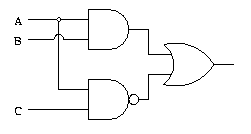
\includegraphics[scale=0.6]{gate}
					\end{center}
					\begin{oneparchoices}
						\choice Signal
						\choice No signal
						\choice Indefinite
					\end{oneparchoices}
					\question A lightyear is the distance light travels in one Earth year. What is 1 light year in kilometers? \\
					\begin{oneparchoices}
						\choice $2.59 \times 10^{10} km$
						\choice $1.58 \times 10^{11} km$
						\choice $2.63 \times 10^{9} km$
						\choice $9.46 \times 10^{12} km$
					\end{oneparchoices}
					\question Water floats on the liquid state of carbon tetrachloride. The two liquids do not mix. A light ray passing from water into carbon tetrachloride has an incident angle of 45.0 degrees and an angle of refraction of 40.1 degrees. If the index of refraction of water is 1.33, what is the index of refraction of carbon tetrachloride?\\
					\begin{oneparchoices}
						\choice 1.60
						\choice 1.49
						\choice 1.21
						\choice 1.46
					\end{oneparchoices}	
					\question What is the magnification of a convex lens if it produces a virtual, 12-cm high image of a 4-cm high object?\\
					\begin{oneparchoices}
						\choice -3
						\choice +3
						\choice $\dfrac{1}{3}$
						\choice -$\dfrac{1}{3}$
					\end{oneparchoices} 
					\question Which of the following is not the result of refraction? 
					\begin{choices}
						\choice A stick immersed in water appears to be broken.
						\choice Formation of images by mirrors.
						\choice The apparent depth of an object in water being smaller than the actual object.
						\choice A star looking higher in the sky than it actually is.
					\end{choices}
					\question  The magnification of a book held 7.50 cm from a 10.0 cm focal length lens was found to be 4.00. What is the magnification for the book when it is held 8.50 cm from the magnifier?\\ 
					\begin{oneparchoices}
						\choice +6.67
						\choice +3.33
						\choice -6.67
						\choice -3.33
					\end{oneparchoices}	
					\question Calculate the power of the mirror formed by the shiny back of a spoon that has a 3.00 cm radius of curvature. \\
					\begin{oneparchoices}
						\choice +66.7 D
						\choice +33.3 D
						\choice -66.7 D
						\choice -33.3 D	
					\end{oneparchoices}
					\question In the figure below, if $\textbf{i}=30^0$(the angle of incidence at A) and $\alpha=95^0$, what is the value of $\textbf{r}'$(the angle of reflection for the reflected ray at B)?
					\begin{center}
						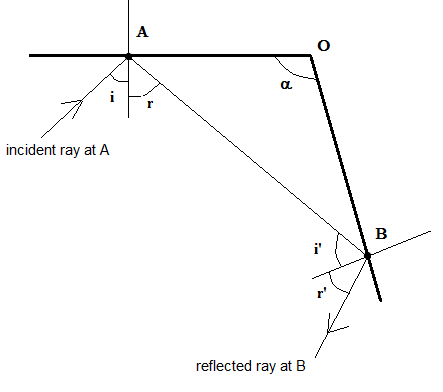
\includegraphics[scale=0.5]{reflection}
					\end{center}
					\begin{oneparchoices}
						\choice $25^0$
						\choice $75^0$
						\choice $65^0$
						\choice $15^0$
					\end{oneparchoices}
				    \question For eye surgery, we use a $193nm$ UV radiation. Assuming the accuracy with which this EM radiation can ablate the cornea is directly proportional to wavelength, how much more accurate can this UV be than the shortest visible wavelength of light($380nm$)?\\
				    \begin{oneparchoices}
				    	\choice 0.508
				    	\choice 1.97
				    	\choice 2
				    	\choice 1.508
				    \end{oneparchoices}
			    	\question If the moon suddenly exploded, how long after the incident will we find out here on Earth if the Moon is on average, $384,400km$ away from Earth?\\
			    	\begin{oneparchoices}
			    	\choice 1.28 s
			    	\choice 2.56 s
			    	\choice 2.4 s
			    	\choice 7 minutes \& 46 seconds	
					\end{oneparchoices}				    
		    		\question Where does an object need to be placed relative to a microscope for its 0.500 cm focal length objective to produce a magnification of -400? \\
		    		\begin{oneparchoices}
		    			\choice 0.510 cm
		    			\choice 0.501 cm
		    			\choice 0.610 cm
		    			\choice 0.499 cm
		    		\end{oneparchoices}
		    		\subsection*{Workout Problems}
					\question Combine thin lens equations to show that the magnification for a thin lens is determined by its focal length and the object distance and give a function that expresses the magnification as a function of the focal 	length and distance of object.\vspace{1.5in}
					\question What power of spectacle lens is needed to correct the vision of a nearsighted person whose far point is 25.0 cm? Assume the spectacle (corrective) lens is held 1.50 cm away from the eye by eyeglass frames.\vspace{1.5in}
					\question A dentist uses a small mirror that gives a magnification of 5.0 when it is held 0.60cm from tooth. 
					\begin{itemize}
						\item What is the radius of curvature of the mirror?\vspace{1.5in} 
						\item What about its power?\vspace{1in}
					\end{itemize}
					\question For an object placed in front of a convex lens such that $d_o=2f$,
					\begin{itemize}
						\item trace the rays and draw the image.\vspace{1in}
						\item show that the image is as far away from the lens as the object is. \vspace{1.5in}
					\end{itemize} 
					\question If a pulsed laser may produce an electromagnetic wave with a maximum electric field strength of  $2.05\times10^{11}V/m$ for a time span of 1.00 ns, determine
					\begin{itemize}
						\item the maximum magnetic field strength in the wave\vspace{1.5in}
						\item the potential difference if it was applied over a distance of 2$\mu$m\vspace{1.5in}
					\end{itemize}
					\subsection*{Extra Credit Problems}
					\question An EM radiation from a 6.00-W laser is concentrated on an area of 0.50$mm^2$, if a static charge moves at a speed of 0.005$c$, what is the maximum force it can feel?\vspace{1in}
					\question Find the power of a lens whose radii are 10cm and 12cm and if it is made of crown glass($n=1.52$)?\vspace{1.5in}
				\end{questions}
				\begin{center}
					\subsection*{Answer Sheet}\vspace{0.5in}
					\begin{tabular}{lllllc}
						1.\noindent\rule{1.5cm}{0.4pt} & 6.\noindent\rule{1.5cm}{0.4pt}  & 11.\noindent\rule{1.5cm}{0.4pt} & 16.\noindent\rule{1.5cm}{0.4pt} & 21.\noindent\rule{1.5cm}{0.4pt} & 26.\noindent\rule{1.5cm}{0.4pt} \vspace{0.5cm} \\ 
						2.\noindent\rule{1.5cm}{0.4pt} & 7.\noindent\rule{1.5cm}{0.4pt}  & 12.\noindent\rule{1.5cm}{0.4pt} & 17.\noindent\rule{1.5cm}{0.4pt} & 22.\noindent\rule{1.5cm}{0.4pt} & 27.\noindent\rule{1.5cm}{0.4pt} \vspace{0.5cm} \\
						3.\noindent\rule{1.5cm}{0.4pt} & 8.\noindent\rule{1.5cm}{0.4pt} & 13.\noindent\rule{1.5cm}{0.4pt} & 18.\noindent\rule{1.5cm}{0.4pt} & 23.\noindent\rule{1.5cm}{0.4pt} & 28.\noindent\rule{1.5cm}{0.4pt} \vspace{0.5cm}\\
						4.\noindent\rule{1.5cm}{0.4pt} & 9.\noindent\rule{1.5cm}{0.4pt} & 14.\noindent\rule{1.5cm}{0.4pt} & 19.\noindent\rule{1.5cm}{0.4pt} & 24.\noindent\rule{1.5cm}{0.4pt} & 29.\noindent\rule{1.5cm}{0.4pt} \vspace{0.5cm}\\
						5.\noindent\rule{1.5cm}{0.4pt} & 10.\noindent\rule{1.5cm}{0.4pt} & 15.\noindent\rule{1.5cm}{0.4pt} & 20.\noindent\rule{1.5cm}{0.4pt} & 25.\noindent\rule{1.5cm}{0.4pt} & 30.\noindent\rule{1.5cm}{0.4pt} \vspace{0.5cm}\\              
					\end{tabular}
				\end{center}
			\end{document}